\section{Result and Discussion}
\label{sec:result-and-discussion}

This section discusses and shows the results from our test and analysis on training humanoid robot model, human model comparison, and also compares their suitability.
All tests were conducted using the Ichiro robot in the \emph{Robot Cerdas} Laboratory with computer specifications as can be seen in Table \ref{tb:computerspecichiro}.
\begin{table}
\caption{Computer specification on Ichiro robot.}
\centering
    \begin{tabular}{|c|c|}
    \hline
    OS      & Ubuntu 20.04.2 LTS \\
    \hline
    CPU     & Intel i5-10210U (8) @ 4.200GHz \\
    \hline
    GPU     & Intel UHD Graphics  \\
    \hline
    RAM     & 3636 MiB \\
    \hline
    \end{tabular}
    \label{tb:computerspecichiro}
\end{table}

\subsection{New Dataset Statistics}
\label{subsec:new-dataset-statistics}

This new dataset is a merge of the HumanoidRobotPose dataset and Ichiro's pose dataset. Figure \ref{fig:nimbro-statistics} shows the statistics for the HumanoidRobotPose dataset and Figure \ref{fig:new-dataset-statistics} shows the statistics for the new dataset.
\begin{figure}[ht]
  \centering
  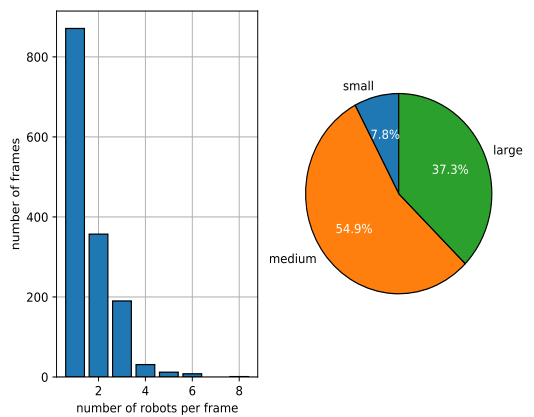
\includegraphics[width=0.4\textwidth]{gambar/old_dataset.png}
  \caption{HumanoidRobotPose Statistics.}
  \label{fig:nimbro-statistics}
\end{figure}
The diversity of the number of robot instances per image is illustrated on the left, and the scale proportions of robot instances is shown on the right. The definition of small, medium, and large scale is identical to the COCO dataset.
Most of the additions (Ichiro's pose dataset) are one robot instance (from approximately 850 to 1700) and few are two instances per image (from approximately 380 to 430) with large scale, i.e., (segment area \textgreater 96\textsuperscript{2}). 
This was based on a system requirement that only need pose estimation for one robot and since the distance between the camera and the robot is not that far, the robot object in the image is mainly on a large scale.
\begin{figure}[ht]
  \centering
  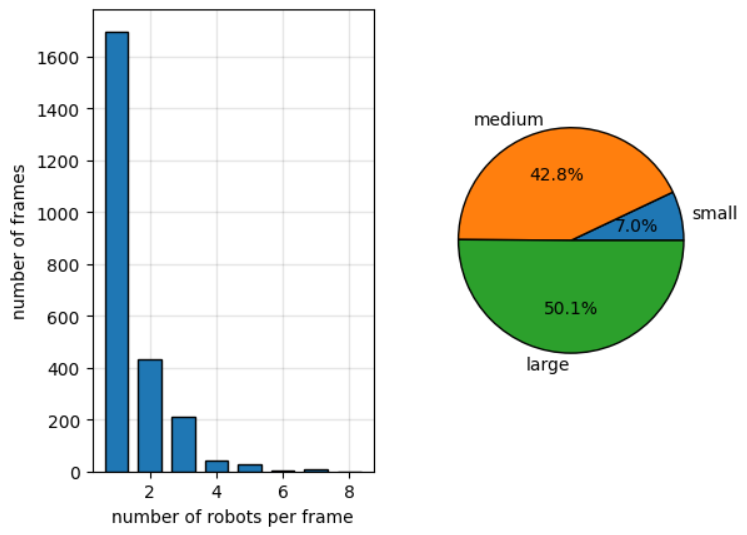
\includegraphics[width=0.4\textwidth]{gambar/new_dataset.png}
  \caption{New Dataset Statistics.}
  \label{fig:new-dataset-statistics}
\end{figure}


\subsection{Robot's Model Training Result}
\label{subsec:robotmodeltrainingresult}

This section shows training graphics, evaluation metrics about three models, and testing we perform such as visualizing detection results and inference time.
Figure \ref{fig:nimbro-training-graphics} and \ref{fig:rcnn-training-graphics} show graphics for training loss (on the left) and validation loss (on the right).
\begin{figure}[ht]
  \centering
  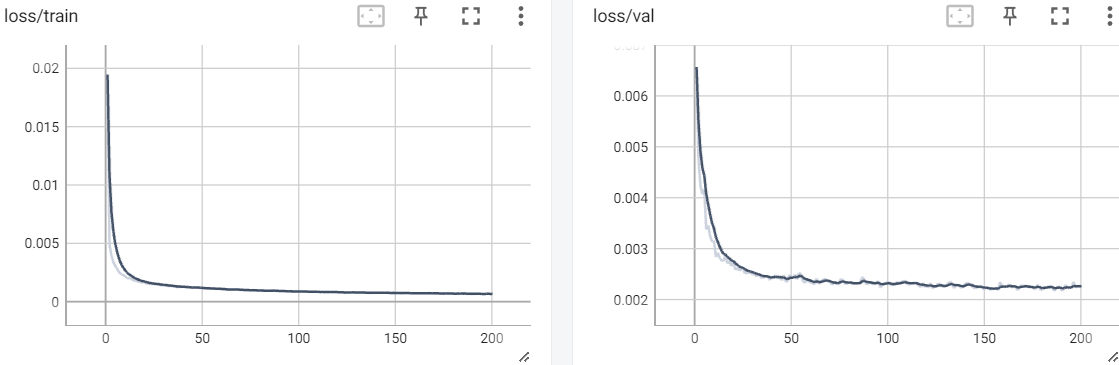
\includegraphics[width=0.48\textwidth]{gambar/loss-nimbro.png}
  \caption{Nimbro Training Graphics.}
  \label{fig:nimbro-training-graphics}
\end{figure}
Training loss and validation loss of NimbRo's model decreased from 0.02 to 0.0006 and 0.0065 to 0.002 respectively. From Figure \ref{fig:rcnn-training-graphics},
we also can know that training loss and validation loss of Keypoint RCNN decreased from 6.991 to 2.634 and 5.926 to 3.439 respectively. Initially, the training loss is high as the model's parameters are randomly initialized,
  and the model has not yet learned to make accurate predictions. As the training progresses, the loss generally decreases, indicating that the model is learning and improving its performance.
The training loss steadily decreases and eventually stabilizes, this indicates the model has converged and training does not need to be continued.
Like training loss, initially, validation loss is relatively high since the model has not been exposed to the validation data. As the model learns from the training data, the validation loss should decrease,
  indicating improved generalization performance. The validation loss steadily decreases and stabilizes in the end.
\begin{figure}[ht]
  \centering
  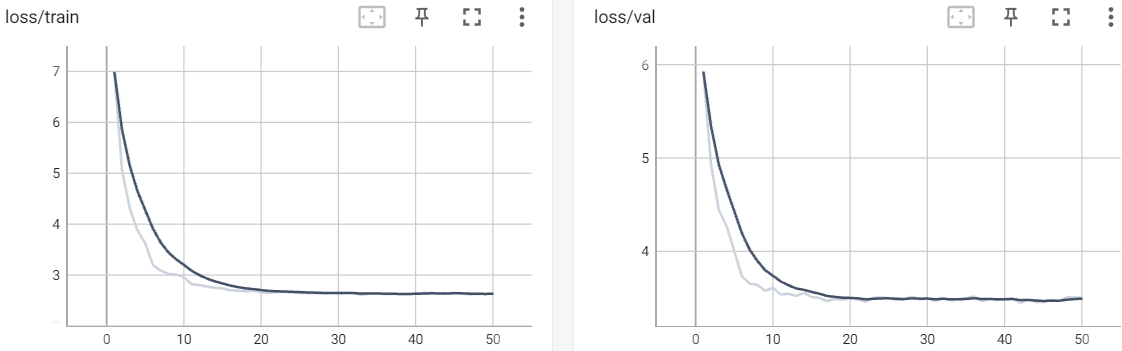
\includegraphics[width=0.48\textwidth]{gambar/loss-rcnn.png}
  \caption{Keypoint RCNN Training Graphics.}
  \label{fig:rcnn-training-graphics}
\end{figure}

For the evaluation metrics, NimbRo's Model and Keypoint RCNN use the Object Keypoint Similarity (OKS) with a per-keypoint constant equal to 0.4 for all keypoints.
YOLO also uses OKS, they follow COCO pose estimation standard evaluation metric.
The results on the test set are reported in Table \ref{tb:result-on-test-set}. It can be seen that Keypoint RCNN outperforms other methods in all metrics except for medium scale.
Moreover, Keypoint RCNN showed the best detection results as shown in Table \ref{tb:robotmodelcomparisondetectionresults}, followed by NimbRo's Model and YOLO-pose.
Lastly, NimbRo's Model is the most likely to be applied to real-time systems because it has the lowest inference time as shown in Table \ref{tb:inference-robot}.
However, since the in PLAY mode, we can do the pose estimation for both human and humanoid robot in the end, not in real-time so the Keypoint RCNN model is suitable for this study.
\begin{table}
  \caption{Inference Time Model Humanoid Robot.}
  \centering
      \begin{tabular}{{|c|c|c|}}
      \hline
      \rowcolor{lightgray}
      \textbf{Model}    & \textbf{PyTorch (s)} & \textbf{OpenVINO (s)}\\
      \hline
      NimbRo's Model & 0.4 - 0.5 & 0.15 - 0.2 \\
      \hline
      RCNN Keypoint  & 3.5 - 4.0 & 1.25 \\
      \hline
      YOLO-pose      & 0.7 - 0.75& 0.27 - 0.3 \\
      \hline
      \end{tabular}
      \label{tb:inference-robot}\\
  \end{table}

\begin{table*}
  \caption{Results on the test set.}
  \centering
      \begin{tabular}{|c|c|c|c|c|c|c|c|c|c|c|} 
      \hline
      \rowcolor{lightgray} \textbf{Model} & \textbf{AP} & \textbf{AP\textsubscript{50}} & \textbf{AP\textsubscript{75}} & \textbf{AP\textsubscript{M}} & \textbf{AP\textsubscript{L}} & \textbf{AR} & \textbf{AR\textsubscript{50}} & \textbf{AR\textsubscript{75}} & \textbf{AR\textsubscript{M}} & \textbf{AR\textsubscript{L}} \\ 
      \hline
      NimbRo's Model        & 0.828       & 0.879                         & 0.840                         & \textbf{0.886}                         & 0.864                        & 0.836       & 0.884                         & 0.849                         & 0.895                        & 0.872 \\
      \hline
      RCNN Keypoint           & \textbf{0.879}       & \textbf{0.936}                         & \textbf{0.904}                         & 0.859                        & \textbf{0.937}                       & \textbf{0.925}       & \textbf{0.973}                         & \textbf{0.944}                         & \textbf{0.936}                        & \textbf{0.955} \\
      \hline
      YOLO-pose           & 0.849       & 0.838                         & -                             & -                            & -                            & 0.814       & -                             & -                             & -                            & - \\
      \hline
      \end{tabular}
      \label{tb:result-on-test-set}\\
  \end{table*}

\begin{table*}
\caption{Robot Model Comparison Detection Results.}
\centering
    \begin{tabular}{|c|c|c|}
    \hline
    \rowcolor{lightgray}
    \textbf{NimbRo}    & \textbf{RCNN} & \textbf{YOLO-pose}\\
    \hline
    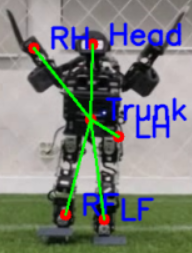
\includegraphics[scale=0.62]{gambar/nimbro-1.png} & 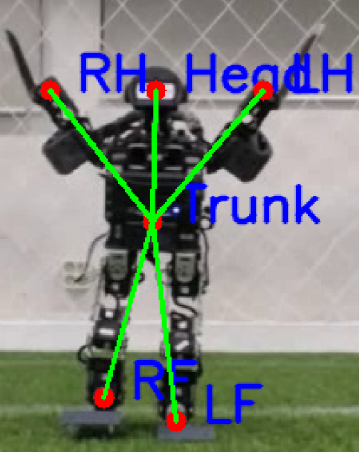
\includegraphics[scale=0.35]{gambar/rcnn-1.png} & 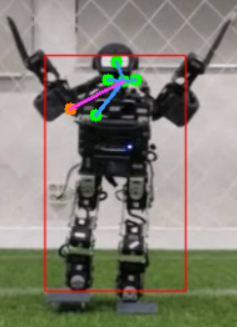
\includegraphics[scale=0.48]{gambar/yolo-1.png} \\
    \hline
    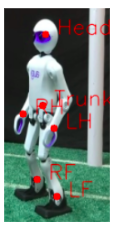
\includegraphics[scale=0.62]{gambar/nimbro-3.png} & 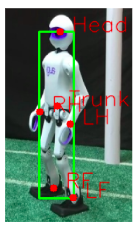
\includegraphics[scale=0.36]{gambar/rcnn-3.png} & 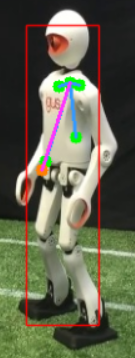
\includegraphics[scale=0.49]{gambar/yolo-3.png} \\
    \hline
    \end{tabular}
    \label{tb:robotmodelcomparisondetectionresults}\\
\end{table*}


\subsection{Human's Model Comparison}
\label{subsec:humanmodelcomparison}

Based on study held by \citet{bazarevsky2020} that compares three different models: BlazePose Lite, BlazePose Full, and OpenPose (body only), they test the models on AR Dataset and Yoga Dataset. As an evaluation metric, they use the Percent of Correct Points with 20\% tolerance (PCK@0.2)
BlazePose shows slightly worse performance than the OpenPose model on the AR dataset but BlazePose Full outperforms OpenPose on Yoga/Fitness use cases.
Note that, in this study, we use BlazePose Full because by default the value of \emph{model complexity} argument is 1 in the \emph{mediapipe.solutions.pose.Pose} API class.
Since in this study, we just need single-person pose detection, MediaPipe should be the best and also a reliable choice.
% \begin{table}
% \caption{Inference Time Model Human.}
% \centering
%     \begin{tabular}{{|c|c|c|}}
%     \hline
%     \rowcolor{lightgray}
%     \textbf{Model}    & \textbf{Inference Time (s)} \\
%     \hline
%     Mediapipe   & 0.15 - 0.2\\
%     \hline
%     OpenPose    & 0.2\\
%     \hline
%     YOLO-Pose   & 0.7 - 0.75\\
%     \hline
%     \end{tabular}
%     \label{tb:inference-human}\\
% \end{table}

\subsection{Comparing the Suitability Between Humanoid Robot Pose and Human Pose}
\label{subsec:comparingsuitability}

By using the method in Subsection \ref{subsec:comparing-keypoints}, we get the result from comparing the human pose and robot pose in percentage terms.
We can see the two figures below, in Figure \ref{fig:comparingb} humans make movement that are more like robot than in Figure \ref{fig:comparinga}.
Therefore, the comparison result of Figure \ref{fig:comparingb} is higher at 91\% than Figure \ref{fig:comparinga} with just 79\%.
This indicates that the system can provide an accurate assessment between the poses of humans and robots.

\begin{figure*}
\centering
\subfloat[Human Image A]{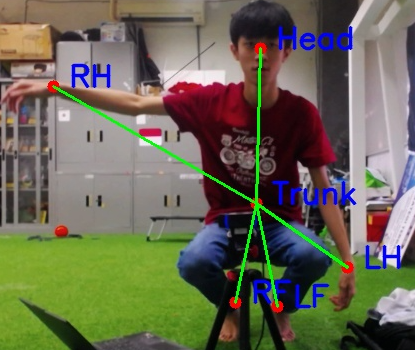
\includegraphics[width=.28\textwidth]{gambar/human_10_result.jpg}
    \label{fig:humanimagea}}
\hfil
\subfloat[Robot Image A]{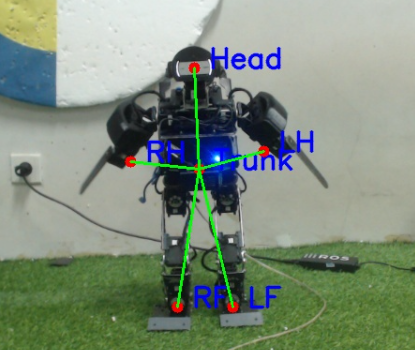
\includegraphics[width=.28\textwidth]{gambar/robot_6_result.jpg}
    \label{fig:robotimagea}}
\caption{Comparing Humanoid Robot Pose and Human Pose.}
\label{fig:comparinga}
\end{figure*}

\begin{figure*}
\centering
\subfloat[Human Image B]{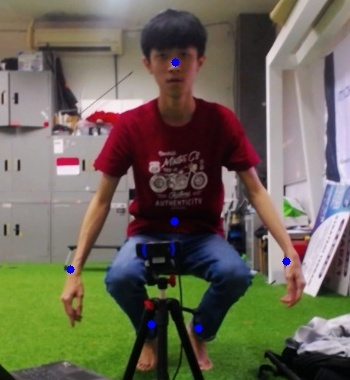
\includegraphics[width=.28\textwidth]{gambar/human_6_result.jpg}
    \label{fig:humanimageb}}
\hfil
\subfloat[Robot Image B]{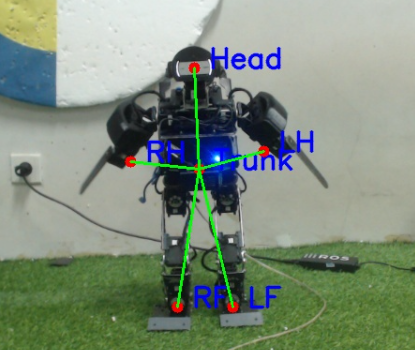
\includegraphics[width=.28\textwidth]{gambar/robot_6_result.jpg}
    \label{fig:robotimageb}}
\caption{Comparing Humanoid Robot Pose and Human Pose.}
\label{fig:comparingb}
\end{figure*}